\documentclass[12pt,twoside,a4paper]{book}
\usepackage[utf8]{inputenc}
\usepackage[spanish]{babel}
\usepackage{graphicx}
\usepackage[dvips]{epsfig}
\usepackage{amssymb}
\usepackage{eurosym}
\usepackage{float}
\usepackage{latexsym}
\usepackage{a4}
\usepackage{xcolor}
\usepackage{listings}
\usepackage{listingsutf8}
\usepackage{enumitem}
\usepackage{hyperref} % menús no pdf pero non leva ben co package galician

\setlist{itemsep=1pt,topsep=1pt}
\addto\captionsgalician{\def\contentsname{Memoria tipo B -- \'{I}ndice xeral }}

\definecolor{backcolor}{rgb}{0.95,0.95,0.92}
\newcommand{\greencolor}{green!70!black}
\lstset{
  caption=\lstname,
  captionpos=b,
  label=lst:code,
  basicstyle=\ttfamily\footnotesize,
  numbers=left,
  commentstyle=\color{gray},
  keywordstyle=\color{blue},
  stringstyle=\color{\greencolor},
  showspaces=false,
  showstringspaces=false,
  showtabs=false,
  tabsize=2,
  keepspaces=true,
  breaklines=true,
  breakatwhitespace=false,
  frame=l,
  % framexleftmargin=8mm,
  % framextopmargin=2pt,
  backgroundcolor=\color{backcolor},
  rulesepcolor=\color{gray!50},
  postbreak=\mbox{\textcolor{red}{$\hookrightarrow$}\space},
  escapeinside={(*@}{@*)}
}
\renewcommand*{\lstlistlistingname}{Índice de Listings}

\lstdefinelanguage{Dockerfile}{
  keywords={FROM, RUN, COPY, ADD, ENTRYPOINT, CMD,  ENV, ARG, WORKDIR, EXPOSE, LABEL, USER, VOLUME, STOPSIGNAL, ONBUILD, MAINTAINER, HEALTHCHECK},
  keywordstyle=\color{blue}\bfseries,
  identifierstyle=\color{black},
  comment=[l]{\#},
  commentstyle=\color{gray}\ttfamily,
  stringstyle=\color{\greencolor}\ttfamily,
  morestring=[b]',
  morestring=[b]"
}

\lstdefinelanguage{docker-compose}{
  keywords={services, depends_on, hostname, image, environment, container_name, ports, volumes, links},
  keywordstyle=\color{blue}\bfseries,
  identifierstyle=\color{black},
  comment=[l]{\#},
  commentstyle=\color{purple}\ttfamily,
  stringstyle=\color{\greencolor}\ttfamily,
  morestring=[b]',
  morestring=[b]"
}

\begin{document}
\pagestyle{empty}
\begin{center}
	{\bf\Large UNIVERSIDAD DE SANTIAGO DE COMPOSTELA}
	
	\vspace{0.5cm}
	
\includegraphics[width=5cm]{figuras/logo_usc.eps}
	
	\vspace{0.5cm}
	{\bf\large ESCUELA TÉCNICA SUPERIOR DE INGENIERÍA}
	
	\vspace{3cm}
	{\bf\LARGE Ciclo completo de CI/CD con Dagger y Kubernetes}
	
\end{center}

\vspace{2cm}
\hspace{4cm}\begin{tabular}{l}
	{\it\Large Autor/a:} \\
	{\bf\Large Daniel Vieites Torres} \\
	~ \\
	{\it\Large Tutores:} \\
	{\bf\Large Pichel} \\
	{\bf\Large Francisco Maseda Muiño} \\
\end{tabular}

\vspace{2cm}
\begin{center}
	{\bf\Large Grado en Ingeniería Informática}
	
	\vspace{0.5cm}
	{\bf\large  2025}
	
	\vspace{0.5cm}
	Trabajo de Fin de Grado presentado en la Escuela Técnica Superior de Ingeniería de la Universidad de Santiago de Compostela para la obtención do Grado en Ingeniería Informática
\end{center}


\cleardoublepage
% \pagestyle{plain}
\pagenumbering{roman}

\includegraphics[width=4cm]{figuras/logo_usc.eps}

\vspace{1cm}
{\bf D. (Nome da titora ou do titor)}, Profesor/a do Departamento de Electrónica e Computación da Universidade de Santiago de Compostela, e {\bf D. (Nome da cotirora ou do cotitor)}, Profesor/a do Departamento de Electrónica e Computación da Universidade de Santiago de Compostela,

\vspace{1cm}
INFORMAN:

\vspace{1cm}
Que a presente memoria, titulada {\it (Título do traballo)}, presentada por {\bf D. (Nome da autora ou do autor do traballo)} para superar os créditos correspondentes ao Traballo de Fin de Grao da titulación de Grao en Enxeñaría Informática, realizouse baixo nosa titoría no Departamento de Electrónica e Computación da Universidade de Santiago de Compostela.

\vspace{1cm}
E para que así conste aos efectos oportunos, expiden o presente informe en Santiago de Compostela, a (Data):

\vspace{2cm}
\begin{tabular}{lll}
	Titor/a, & Cotitor/a, & Alumno/a, \\
	~ \\
	~ \\
	~ \\
	~ \\
	~ \\
	~ \\
	~ \\
	(Nome do titor/a) & (Nome do cotitor/a) & (Nome do alumn/a)
\end{tabular}

 % paxina de certificación (optativa)
% \cleardoublepage
% \pagestyle{plain}
\chapter*{Agradecementos}
Se se quere pór algún agradecemento, este vai aquí.

 % paxina de agradecementos (optativa) 
% \cleardoublepage
\pagestyle{plain}
\chapter*{Resumen}

Ante la creciente complejidad de los flujos DevOps, resulta conveniente identificar herramientas de \textit{Continuous Integration/Continuous Delivery} (CI/CD) que unifiquen los \textit{pipelines} y reduzcan los costes de mantenimiento. Este trabajo investiga si Dagger, un motor programable basado en contenedores, puede simplificar y acelerar la integración y entrega continuas frente a los métodos convencionales predominantes.

Se construyó un \textit{monorepo} con una aplicación de prueba (\textit{frontend}: Vue + Typescript; \textit{backend}: Typescript; MongoDB) y se diseñaron e implementaron dos módulos de Dagger para los ciclos de CI y CD, empleando el SDK que proporciona Dagger para el lenguaje de programación Go. Además, se desplegó la aplicación en tres \textit{clusters} de KinD, gestionados por ArgoCD bajo filosofía GitOps, con la infraestructura definida mediante Helm y Kubernetes.

La evaluación cuantitativa incluyó una prueba en la que se ejecutó la función \texttt{endtoend} del módulo de CI. Esta mostró una reducción del tiempo de ejecución del 40\% cuando los parámetros de entrada cambiaban entre ejecuciones, y del 94\% cuando los parámetros permanecían sin cambios. Esto es gracias al sistema de gestión de caché nativo de Dagger. El análisis cualitativo destacó ventajas en cuanto al mantenimiento, la portabilidad (ejecución sobro \textit{runtime} OCI), la reproducibilidad y la escalabilidad, frente a una curva de aprendizaje moderada.

En conclusión, Dagger se posiciona como una alternativa sólida para estandarizar y modernizar los ciclos de vida del \textit{software}, facilitando la integración continua y reduciendo la dependencia de \textit{scripts} heterogénos. Se sugiere como mejora futura la validación del funcionamiento de los módulos en \textit{clusters} gestionados en la nube.
 % páxina de resumo (optativa) 

\cleardoublepage
\pagestyle{plain}
\tableofcontents
\listoffigures
\listoftables
\lstlistoflistings

% Agora incluimos os capítulos. Cambiamos a numeración e as cabeceiras
\cleardoublepage
\pagenumbering{arabic}
\setcounter{page}{1}
\pagestyle{headings}
\chapter{Introdución}

% Obxectivos Xerais, Relación da Documentación que conforma a Memoria, Descrición do Sistema, Información Adicional de Interese (métodos, técnicas ou arquitecturas utilizadas, xustificación da súa elección, etc.).

\section{Objetivos generales}

% qué problema se resuelve y cuál es el propósito de este trabajo

\subsection*{Objetivos principales}

En este trabajo se pretende demostrar y evaluar la viabilidad, eficiencia y flexibilidad de Dagger\cite{dagger} como motor de CI/CD (\textit{Continuous Integration}/\textit{Continuous Delivery})\cite{ci,cd}, con el fin de estandarizar y modernizar los ciclos de vida del desarrollo de software.

No solo se va a utilizar Dagger como complemento del ciclo de desarrollo de una aplicación, sino que se va a comparar con la no utilización de este. Se evaluarán las ventajas que tiene su uso frente a métodos convencionales, entre las que destacarán la gestión de caché y el uso de contenedores.

Se van a proporcionar ejemplos de módulos creados con Dagger, los cuales estarán especialmente diseñados para cumplir los ciclos tanto de CI  como de CD  de una aplicación \textit{dummy}. De esta manera se podrá comprobar que este mismo proceso se puede llevar a cabo para cualquier aplicación, y de una manera sencilla.

\subsection*{Objetivos secundarios}

Para lograr los objetivos principales es necesario llevar a cabo varios pasos:
\begin{itemize}
  \item Creación de un monorepo\cite{monorepo} en GitHub.

    Todo el código principal se almacenará en un mismo repositorio. De esta manera se evitarán complicaciones debido a la gestión de dependencias de cada una de las partes de la aplicación. Permitirá controlar todo el código fuente de una manera más sencilla al tratarse de un proyecto relativamente pequeño.
  \item Diseño y creación de una aplicación \textit{dummy}.

    Es necesario una aplicación sobre la que realizar los ciclos de CI/CD. Esta consistirá en una página web (frontend) de gestión de un zoo, la cual realizará peticiones a una API (backend) que estará conectada a una base de datos.
  \item Implementación de un \textit{pipeline} CI/CD.

    Se creará un módulo de Dagger para cada uno de los procesos (CI y CD). El módulo de CI permitirá desde compilar la aplicación, hasta publicar las imágenes de Docker y los paquetes NPM de cada una de las partes. Por otro lado, el módulo de CD será el encargado de utilizar esas imágenes que se han publicado previamente y desplegar la aplicación en el entorno correspondiente.
  \item Entorno orquestado.

    El \textit{pipeline} de CD termina con el despliegue de la aplicación sobre Kubernetes\cite{kubernetes}, utilizando Helm\cite{helm}. Esto permite levantar la aplicación en el entorno que le corresponda, según el estado en el que se encuentra cada versión.

  \item Análisis comparativo

    Finalmente, se realiza un análisis de las ventajas que ofrece Dagger frente a métodos convencionales.
\end{itemize}

\section{Relación de la documentación}

\begin{itemize}
  \item Capítulo 1: Introducción.

    Este capítulo, en el cual se describen la finalidad del proyecto, las tecnologías a utilizar, de manera breve; y la estructura, a grandes rasgos, del trabajo en sí.

  \item Capítulo 2: Estado del arte y fundamentos teóricos.

    En el segundo capítulo se detallan los conceptos más importantes de CI/CD. Además, se estudia la evolución de las herramientas DevOps\cite{devops}, incluyendo Dagger como una de las últimas y más innovadoras herramientas en este sector, y se compara con las otras tecnologías.
  \item Capítulo 3: Diseño y arquitectura del sistema.

    Aquí se describen las tecnologías utilizadas para implementar la aplicación \textit{dummy}. También se explica cómo se ha organizado la infraestructura de despliegue.
  \item Capítulo 4: Implementación del \textit{pipeline} con Dagger.

    Aquí se indican los pasos que se han dado para crear los \textit{pipelines} con Dagger, utilizando el SDK para definirlos como código. Este es el núcleo del proyecto.
  \item Capítulo 5: Pruebas y resultados.

    En este capítulo se presentan las pruebas que se han llevado a cabo. Se habla de las dificultades que se han tenido, así como de las ventajas que ofrece Dagger frente a otras tecnologías, aportando comparaciones cuantitativas y cualitativas.
  \item Capítulo 6: Conclusiones y líneas futuras.

    Finalmente, se resumen los hechos que se han obtenido, se valora el resultado final del uso de Dagger y se indica si ha cumplido con las expectativas. Además, se añaden puntos de mejora o extensiones del proyecto.
\end{itemize}

\cleardoublepage
\chapter{Estado del arte y fundamentos teóricos}

Antes de empezar a escribir código, se deben entender los conceptos fundamentales que permitirán llevar a cabo este trabajo.

Lo que se intenta mejorar utilizando Dagger es el ciclo completo de CI/CD de una aplicación. Por lo tanto, es fundamental definir los conceptos de \textit{Continuous Integration} y el \textit{Continuous Delivery}. Una vez se comprenda a qué se refieren esos términos, se podrán entender los métodos y tecnologías convencionales que permiten implementar dichos procesos. Será entonces cuando se pueda introducir Dagger, un método innovador para realizar \textit{pipelines}, el cual aporta muchas ventajas y se comparará con otras tecnologías disponibles en el sector.

\section{CI/CD}

CI/CD son las siglas de \textit{Continuous Integration}/\textit{Continuous Delivery}, o en casos más específicos, este último también se puedo conocer como \textit{Continuous Deployment}.

Se trata de un conjunto de pasos automatizados, utilizados en el desarrollo de software para llevar el código desde su implementación inicial hasta el despliegue de la aplicación. Estos pasos incluyen:

\begin{itemize}
  \item Integración de cambios en el código.
  \item La compilación de la aplicación con los cambios realizados.
  \item Realización de pruebas.
  \item Creación y publicación de imágenes de Docker y paquetes NPM.
  \item Despliegue de la aplicación (modelo \textit{push}\cite{push})
\end{itemize}

\subsection*{\textit{Continuous Integration}}

Se basa en la integración de código de manera constante, día a día, en un repositorio compartido por programadores. Cada uno de los programadores realiza cambios en el código y lo integra en el repositorio. Una vez se realizan cambios, estos deben pasar una serie de pruebas para que se incluyan definitivamente en el código fuente de la aplicación (Fig. \ref{ci}).

\begin{figure}
  \centerline{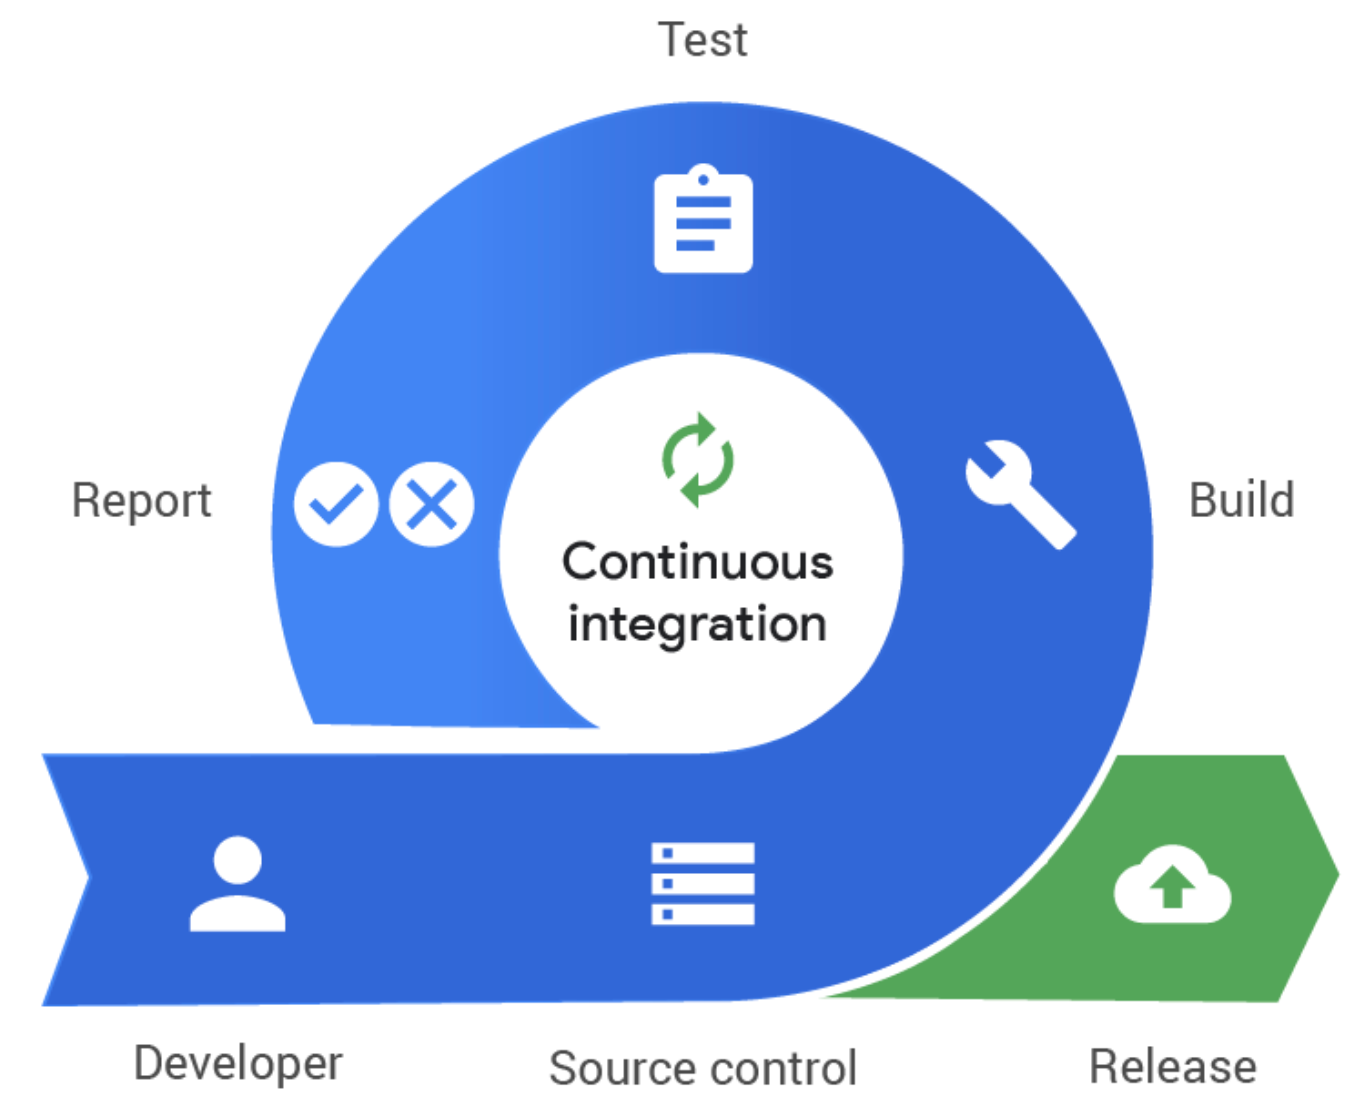
\includegraphics[width=10cm]{figuras/ci}}
  \caption{Proceso de integración continua.\cite{img.ci}}
  \label{ci}
\end{figure}

Desde hace años se utiliza un sistema de control de versiones para gestionar el código de cualquier proyecto. Este tipo de herramientas permite a un equipo controlar el estado del código en cada momento, siendo capaces de conocer el historial de los cambios realizados, saber quién ha hecho cada cambio y tener la capacidad de revertir alguna modificación en el caso de ser necesario. La herramienta de control de versiones más utilizada hoy en día, y la que se utiliza en este proyecto, es Git\cite{git}.

La integración de código en un repositorio no se trata simplemente de modificar una porción de un archivo y subirlo. El código debe ser probado antes de incluirlo completamente en el núcleo de la aplicación. Durante el proceso de integración continua, cada vez que se modifica algo de código, se debe:

\begin{itemize}
  \item Construir la aplicación.
  \item Pasar pruebas de funcionalidad.
  \item Pasar a través de un análisis del propio código (\textit{linting}).
  \item Reportar cualquier error en el caso de que exista.
\end{itemize}

Todo lo anterior se debe realizar de manera automatizada, con el fin de integrar el código modificado en la aplicación lo más rápido posible.

\section{Métodos convencionales}

Como cabe esperar, los pasos mencionados anteriormente que forman parte de la integración continua van a depender del tipo de aplicación que se esté construyendo, y de las tecnologías que se estén utilizando. Además, esta secuencia de acciones pueden incluir unos pocos comandos en trabajos o proyectos sencillos, o necesitar varios \textit{scripts} complejos en el caso de aplicaciones más avanzadas. Por lo tanto, es necesario tener una herramienta que permita realizar los pasos mencionados anteriormente, sin la necesidad de memorizar o saber a ciencia cierta cada uno de los comandos o scripts que hay que ejecutar para comprobar que el código de la aplicación es correcto.

Para ello existe \texttt{make}\cite{make}, una aplicación de línea de comandos que permite definir bloques de comandos o reglas, aportando a cada bloque un nombre u objetivo que se pretende obtener ejecutando dicha regla. Se suele crear un archivo llamado \texttt{Makefile} para definir todas las reglas que se precisen.

\begin{lstlisting}[language=make,label=lst:make]{Makefile para compilación de un programa en C}
# Compiler
CC = gcc

# Compiler options
CFLAGS = -Wall -g

# Final executable name
TARGET = my_program

# The object files (.o) needed by the program
# Make infers automatically that .o depends on the corresponding .c
OBJS = main.o hello.o

# --- Rules ---

# The first rule is the one executed by default with "make"
# It declares that to create the TARGET, it needs the OBJS
$(TARGET): $(OBJS)
  $(CC) $(CFLAGS) -o $(TARGET) $(OBJS)

# ".PHONY" tells Make that "clean" is not a file
.PHONY: clean
clean:
  rm -f $(TARGET) $(OBJS)
\end{lstlisting}

Un ejemplo muy típico de compilación de un programa escrito en \texttt{C} sería el que se puede observar en el Listing \ref{lst:make}.

Sin embargo, en este trabajo se utiliza una versión más nueva y polivalente llamada \texttt{just}\cite{just}. Este software tiene la misma finalidad que \texttt{make}, ejecutar comandos específicos de un proyecto. Pero este incluye muchas más funcionalidades, entre las cuales destacan:

\begin{itemize}
  \item Poder pasar parámetros a las ``recetas'' (las ``reglas'' en \texttt{make}).
  \item Crear aliases para las recetas.
  \item Cargar archivos \texttt{.env}.
  \item Poder definir recetas como scripts en el lenguaje que se prefiera, simplemente añadiendo el \textit{shebang}\cite{shebang} correspondiente.
  \item Ser capaz de ser invocado desde cualquier subdirectorio.
\end{itemize}

\begin{lstlisting}[label=lst:just]{Extracto de justfile utilizado en el proyecto}
# --- ALIASES ---
# Defines shortcuts (aliases) for longer commands.
alias dv := down_vol

# --- DEFAULT RECIPE ---
# This is the recipe that runs if you just type 'just' in the
# terminal.
# By default, it invokes the 'just -l' recipe, which lists all
# available recipes.
# The '_' prefix indicates that it is a helper recipe, not
# intended to be called directly by the user.
_default:
  just -l

# --- INTERNAL (PRIVATE) RECIPES ---
_build_zoo_base:
  #!/usr/bin/env bash
  if [[ "$(docker images -f reference=zoo-base | wc -l | xargs)" != "2" ]]
  then
    docker build --target base -t zoo-base .
  fi

# Accepts two parameters: 'entrypoint' and 'command'.
_run entrypoint command:
  # '@' at the beginning of a command line prevents 'just' from
  # printing the command before executing it.
  @just _build_zoo_base
  docker run --rm -w /app -v $PWD:/app --env-file .env --entrypoint={{entrypoint}} zoo-base {{command}}

# --- PUBLIC RECIPES ---
init:
  @just _run "yarn" "install"

down_vol:
  docker compose down -v
\end{lstlisting}

Como se puede comprobar en el Listing \ref{lst:just}, el archivo de configuración de \texttt{just}, en este caso nombrado habitualmente \texttt{justfile}, tiene una estructura similar a la de un \texttt{Makefile}. La diferencia principal es que los nombres de las recetas no hacen referencia a un archivo objetivo que se supone que se debe crear al ejecutar el bloque de comandos, sino que se trata simplemente del nombre de la receta.

\section{Dagger}

\cleardoublepage
\chapter{Diseño y arquitectura del sistema}

\section{Estructura general}

El código del trabajo y todo lo que abarca se encuentra almacenando en \href{https://github.com/orgs/vieites-tfg/repositories?type=source}{GitHub}. Se han creado los repositorios necesarios en una misma organización de GitHub.

Entre los repositorios creados se pueden encontrar:

\begin{itemize}
  \item \texttt{zoo}.

    Este es el repositorio principal. Se trata de un \textit{monorepo}\cite{monorepo}, en el que se encuentra implementado todo el código necesario dentro del presente trabajo de investigación. En el repositorio se encuentran:
    \begin{itemize}
      \item La aplicación de prueba sobre la que se apoya el proyecto, y que da nombre al repositorio, debido a que se trata de una aplicación de gestión de un zoo.
      \item Los módulos de Dagger para realizar los ciclos de CI y CD.
      \item Otros archivos, como \textit{scripts} y archivos de configuración.
    \end{itemize}

  \item \texttt{helm-repository}.

    Este repositorio alberga las Charts de Helm que definen la estructura necesaria para desplegar la aplicación de prueba.

  \item \texttt{state}.

    Se trata del repositorio que, siguiento el enfoque GitOps, almacena los valores que poblarán los recursos de Kubernetes según el entorno en el que se despliegue la aplicación. Además, en este repositorio también existe una rama de despliegue, de la cual ArgoCD lee los manifiestos de los recursos que debe desplegar para cada uno de los entornos.
\end{itemize}

En la Figura \ref{fig:ghorg} se muestra un diagrama de la disposición de los repositorios y la relación entre ellos.

\begin{figure}[h]
  \centerline{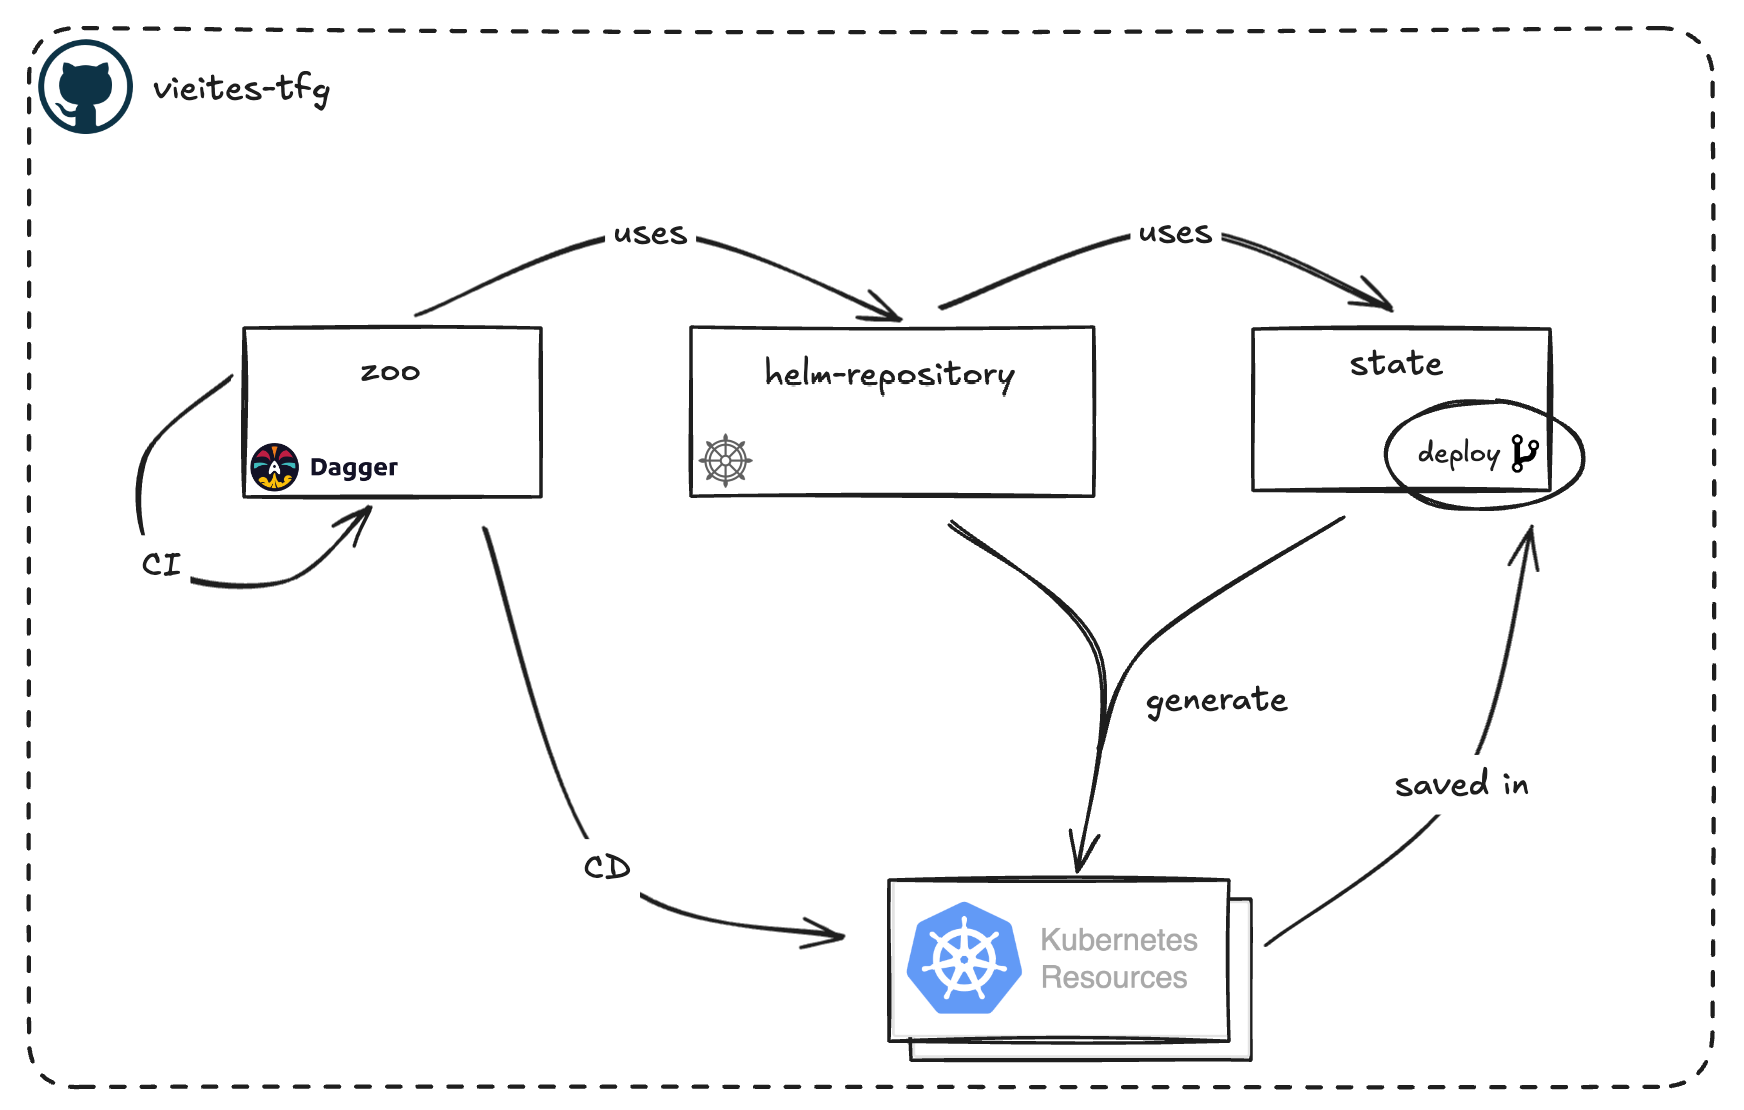
\includegraphics[width=14cm]{figuras/vieites-tfg}}
  \caption{Diagrama de la organización de GitHub. Imagen creada con \href{https://excalidraw.com}{excalidraw.com}.}
  \label{fig:ghorg}
\end{figure}

\section{zoo}

Como se ha comentado anteriormente, el repositorio \texttt{zoo} está estructurado como un \textit{monorepo}. Un \textit{monorepo} es un repositorio con diferentes proyectos, los cuales se encuentran interrelacionados de una manera bien definida. A lo largo de esta sección se justifica la elección de este tipo de estructura, a la vez que se explica cómo están implementados las diferentes piezas de software.

\subsection*{Aplicación de prueba}

La primera razón para escoger un \textit{monorepo} como estructura del repositorio es el hecho de querer crear una aplicación relativamente pequeña, una página web que consta de un \textit{frontend} y un \textit{backend} (se hará referencia a estos como ``paquetes'' a partir de ahora). Por lo tanto, se hace más sencillo gestionar estos dos paquetes si se ubican en un único repositorio.

Otra ventaja de utilizar un \textit{monorepo} tiene que ver con el \textit{software} utilizado para crear los paquetes de la aplicación de prueba. Ambos se implementan utilizando Node.js, en lenguaje Typescript\cite{ts}. Los paquetes tienen dependencias propias, y se puede dar el caso de que ambos utilicen una o varias dependencias iguales. Usar un \textit{monorepo} permite tener esas dependencias en un mismo lugar, evitando su duplicado. Con esto se consigue reducir el tiempo de construcción de los paquetes.

Sin embargo, es necesaria una herramienta que permita manejar los paquetes de manera independiente. Alguno de los motivos para tener esta preferencia pueden ser: que haya dos equipos de desarrolladores, uno para cada paquete; o que se quiera publicar versiones, hacer tests, u otro tipo de tarea sobre cada paquete por separado. La herramienta que se utiliza en este Trabajo de Fin de Grado se llama Lerna\cite{lerna}. Este \textit{software} está específicamente diseñado para gestionar \textit{monorepos} de proyectos de Node.js. Entre las ventajas que proporciona se encuentran:

\begin{itemize}
  \item Gestión de tareas locales.
  \item Cacheo local de salidas de comandos, con posibilidad de que dicha caché sea compartida entre entornos, por ejemplo, con agentes de CI.
  \item Detección de paquetes afectados por cambios en el código.
  \item Análisis de la estructura del proyecto.
\end{itemize}

Por los beneficios anteriormente comentados, y más, es por lo que se ha elegido esta herramienta para gestionar el \textit{monorepo}.

En cuanto a las tecnologías que se utilizan en la aplicación, ya se ha mencionado Typescript como lenguaje principal. Este lenguaje permite tener un sistema tipado, lo cual puede ser útil para detectar muchos errores comunes mediante el análisis estático en tiempo de construcción. Esto reduce las posibilidades de errores en tiempo de ejecución.

El \textit{backend} está completamente desarrollado utilizando dicho lenguaje. Su funcionalidad es proporcionar una API REST que el \textit{frontend} pueda utilizar para realizar cambios en la base de datos. Se usa MongoDB\cite{mongodb} como base de datos debido a que es fácil de gestionar y porque solo se almacena información sobre animales, sin ningún tipo de relación entre ellos, en una única tabla o documento de la base de datos.

El \textit{frontend} se ha implementado utilizando Vue.js\cite{vue}, un \textit{framework} que permite construir interfaces web mediante componentes reactivos. Se ha escogido este frente a otras opciones debido pequeña curva de aprendizaje inicial gracias a su API intuitiva. Además, el propio \textit{framework} está construido utilizando Typescript, por lo que tiene compatibilidad de primera clase con este lenguaje.

En la Figura \ref{fig:app} se puede ver un diagrama que muestra cómo es la comunicación entre los paquetes de la aplicación, y con la base de datos, junto con las tecnologías que se utiliza en cada uno de ellos.

\begin{figure}
  \centerline{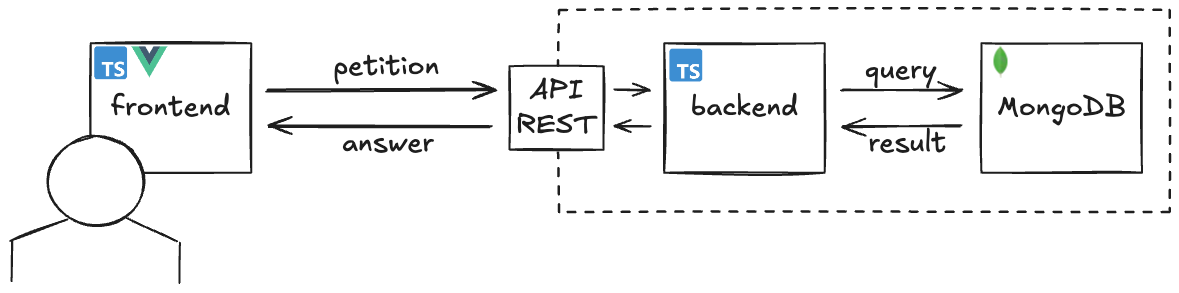
\includegraphics[width=15cm]{figuras/app}}
  \caption{Comunicación entre paquetes de la aplicación. Imagen creada con \href{https://excalidraw.com}{excalidraw.com}.}
  \label{fig:app}
\end{figure}

\subsection*{Módulos de Dagger}

Se integran también en el repositorio los módulos de Dagger de CI y de CD. Estos módulos se incluyen en el \textit{monorepo} para facilitar la referencia a los paquetes que constituyen la aplicación de prueba. Además, resulta lógico que se ubiquen en el mismo lugar una aplicación y las herramientas que permiten su evolución, como son cualquier tipo de \textit{software} que realice las funciones de CI y de CD.

Ambos módulos se realizan utilizando el SDK del lenguaje Go que proporciona Dagger. Se ha escogido este lenguaje debido al conocimiento previo que ya se tenía de este. Además, es el lenguaje en el que está implementado el propio Dagger.

Uno de los módulos se encarga del ciclo de CI, es decir, de realizar los tests de la aplicación, del \textit{linting} o análisis del código en sí, y de la publicación de imágenes de Docker y paquetes NPM. Está organizado de manera que se pueden gestionar cada uno de los paquetes de la aplicación de manera independiente. Esto también es posible gracias al uso de Lerna, que ya se ha comentado anteriormente.

El segundo de los módulos, el de CD, realiza la tarea de publicación de los recursos de Kubernetes, los cuales son posteriormente obtenidos por ArgoCD para su despliegue completo. Esto se consigue haciendo uso de los repositorios \texttt{helm-repository} y \texttt{state}, en los cuales se almacenan las Charts de Helm y los valores que pueblan dichas Charts, respectivamente.

Se detalla más profundamente la implementación de los módulos de Dagger en el Capítulo \ref{chap:dagger}.

\subsection*{Creación y configuración de los \textit{clusters}}
\label{subsec:clusters}

La fase final del ciclo de una aplicación es el despliegue. En este Trabajo de Fin de Grado se levantan tres \textit{clusters} de KinD de manera local. Estos son los lugares en los que se despliega la aplicación. Generalmente se tienen diferentes \textit{clusters} con el fin de probar la aplicación en entornos distintos antes de desplegarla en el principal, que sería el de producción. El hecho de crearlos todos localmente hace que sean más sencillas las pruebas relacionadas con el despliegue. En equipos de desarrollo reales, los entornos de producción se encuentran en la nube. Sin embargo, sí que se pueden llegar a tener entornos locales para realizar pruebas de la aplicación.

Los \textit{clusters} se crean con el \textit{script} que se muestra en el Listing \ref{lst:create-clusters} (se han puesto comentarios en vez de código en algunas partes para reducir su tamaño, a modo de pseudocódigo). Este \textit{script} está escrito para funcionar en sistemas UNIX, en Bash, por lo que es un requisito utilizar un sistema operativo como MacOS o una distribución de Linux para probar el \textit{script}. No funcionará en un sistema operativo Windows. A modo de resumen del \textit{script}:

\begin{longlisting}
  \begin{minted}{bash}
# Variables globales
# ---

for ENV in "${ENVS[@]}"; do
  case "${ENV}" in
    dev)
      BANNER_TEXT="We are in DEV";;
    # ... otros entornos
  esac

  CONTEXT="kind-${ENV}"

  kind create cluster --config "${CLUSTER_DIR}/kind_${ENV}.yaml"

  kubectl apply -f "${INGRESS_MANIFEST}" --context "${CONTEXT}"
  # Se espera a que se construya

  kubectl create namespace argocd || true

  cat "${SOPS_DIR}/age.agekey" |
    kubectl create secret generic sops-age -n argocd \
    --context ${CONTEXT} --from-file=keys.txt=/dev/stdin

  # Se descarga el repositorio de la Chart
  helm install argocd argo/argo-cd -n argocd \
    -f argo/values.yaml \
    # ... otros *flags*

  # Se espera a que se instale la Chart de Argo

  kubectl apply -f "${ARGO_DIR}/argo_${ENV}.yaml" \
    --context "${CONTEXT}"
  # Se espera a que se apliquen los cambios

  # Se aplica el banner a la interfaz de Argo

  # Se obtiene la clave inicial del usuario "admin" y se muestra
  # por pantalla
  PASSWORDS+="${current_pass}"
done

printf "${PASSWORDS}"
\end{minted}
\caption{Script de creación de los clusters. También referenciado en la Sección \ref{sec:secrets}.}
\label{lst:create-clusters}
\end{longlisting}

\begin{itemize}
  \item Se crean tres \textit{clusters} con su configuración específica. Se puede ver el archivo de configuración del \textit{cluster} de \texttt{dev} en el Listing \ref{lst:conf-cluster}.
  \item Se instala en cada \textit{cluster} un controlador de Ingress, lo cual permitirá acceder a la aplicación a través de una URL customizada desde el exterior.

\begin{listing}[!ht]
  \begin{minted}{yaml}
kind: Cluster
apiVersion: kind.x-k8s.io/v1alpha4
name: dev
networking:
  apiServerPort: 6443
nodes:
- role: control-plane
  kubeadmConfigPatches:
  - |
    kind: InitConfiguration
    nodeRegistration:
      kubeletExtraArgs:
        node-labels: "ingress-ready="
  extraPortMappings:
  - containerPort: 80
    hostPort: 8080
    protocol: TCP
  - containerPort: 443
    hostPort: 8443
    protocol: TCP
  \end{minted}
  \caption{Configuración del cluster de dev}
  \label{lst:conf-cluster}
\end{listing}

  \item Se incluye como Secret de Kubernetes el valor de la clave de cifrado que permite desencriptar los secretos. El proceso de creación de cifrado y descifrado se explica en la Sección \ref{subsec:secretos}.
  \item Se instala la Chart de Helm de ArgoCD. A esta Chart se le pasan una serie de valores, de los cuales se habla en la Sección \ref{subsec:secretos}. Más información sobre cómo acceder a la interfaz de ArgoCD en el Apendice \ref{chap:usuario}.
  \item Se aplica la configuración específica de ArgoCD para el entorno que se está creando. Se puede ver la configuración para ArgoCD en el entorno de \texttt{dev} en el Listing \ref{lst:conf-argo}. En dicha configuración se indica el repositorio, la ruta desde la raíz donde se encuentran los recursos y la rama de donde ArgoCD debe obtener los archivos que definen los recursos que se van a desplegar.

\begin{listing}[!ht]
  \begin{minted}{yaml}
apiVersion: argoproj.io/v1alpha1
kind: Application
metadata:
  name: app-dev
  namespace: argocd
spec:
  project: default
  source:
    repoURL: 'https://github.com/vieites-tfg/state.git'
    path: dev
    targetRevision: deploy
  destination:
    server: 'https://kubernetes.default.svc'
    namespace: dev
  syncPolicy:
    automated:
      prune: true
      selfHeal: true
    syncOptions:
      - CreateNamespace=true
    \end{minted}
    \caption{Configuración de ArgoCD en dev}
    \label{lst:conf-argo}
\end{listing}

  \item Se añade un banner en la parte superior de la interfaz para distinguir cada uno de los \textit{clusters}.
  \item Se muestra la contraseña del usuario \texttt{admin}, para poder hacer \textit{log in} a través de la interfaz de ArgoCD.
\end{itemize}

En la Figura \ref{fig:clusters} se puede observar cómo se sincroniza ArgoCD, en cada uno de los \textit{clusters}, con el repositorio de estado. ArgoCD reacciona cada vez que se realizan cambios en el directorio que le corresponde, dentro de la rama de despliegue del repositorio \texttt{state}. En ese momento, obtiene de nuevo todos los archivos de definición de los recursos y se sincroniza con el estado deseado.

\begin{figure}
  \centerline{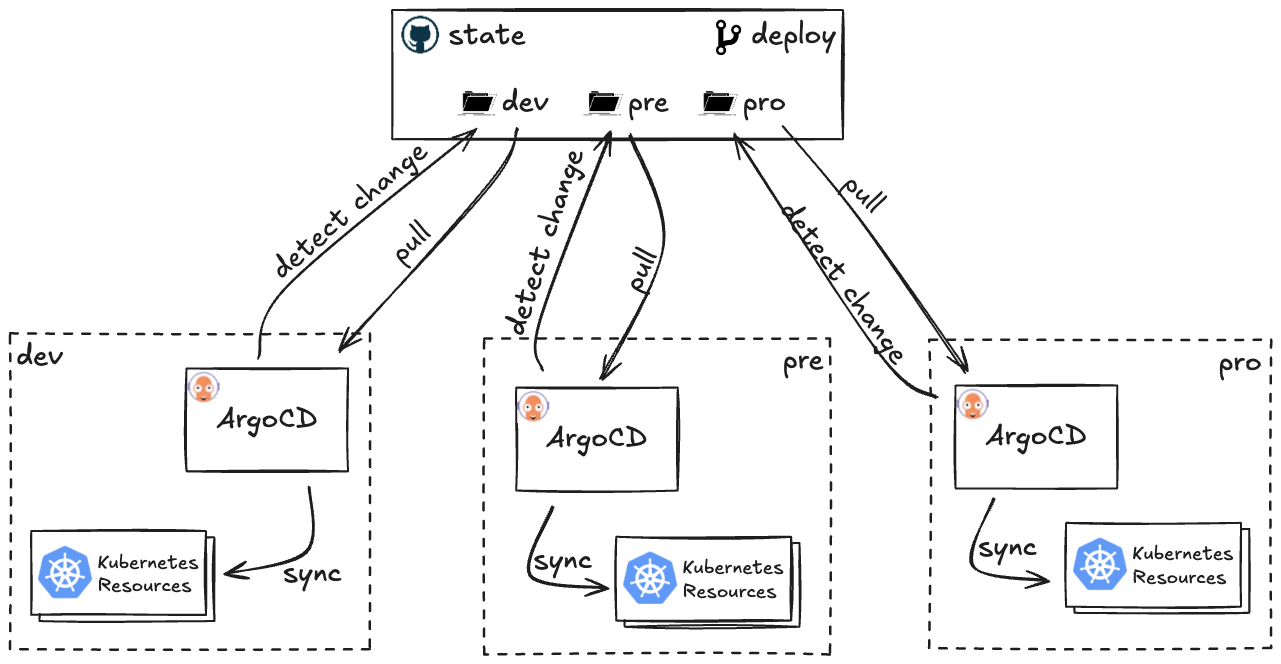
\includegraphics[width=15cm]{figuras/clusters}}
  \caption{Clusters y comunicación con el repositorio de estado. Imagen creada con \href{https://excalidraw.com}{excalidraw.com}.}
  \label{fig:clusters}
\end{figure}


\subsection*{Gestión de secretos}
\label{subsec:secretos}

La aplicación de prueba consta de una base de datos, la cual tiene usuario y contraseña. Este es un ejemplo de datos que es necesario almacenar como un secreto o Secret de Kubernetes. Debido a que se está utilizando un método \textit{pull}\cite{pull} de despliegue de la aplicación; es decir, la herramienta que realiza el despliegue, ArgoCD, ``tira'' (hace \textit{pull}) del repositorio que le indicamos como objetivo; es necesario almacenar en el repositorio los secretos encriptados previamente. Esto es una buena práctica para evitar que se filtren sin querer los datos al exterior, aunque el repositorio sea privado.

Existe un apartado completamente dedicado a como se realiza la gestión de secretos en la Sección \ref{sec:secrets}. 

\subsection*{Función de cada \textit{cluster} y promoción de entornos}
\label{subsec:cluster-func}

A continuación se explica para qué se utiliza cada \textit{cluster} y cuál es el proceso de despliegue de la aplicación en cada uno de los entornos.

\begin{itemize}
  \item \texttt{dev}.

    Se trata del \textit{cluster} de desarrollo. En este se despliega la aplicación en el momento en el que se añade una nueva funcionalidad, ya sea en el \textit{frontend} o en el \textit{backend}. Esto implica, en términos de GitHub:

    \begin{enumerate}
      \item Crear una \textit{Pull Request} (PR) en la que se implementa la nueva funcionalidad. Esta debe ser lo más reducida posible, cumpliendo con la filosofía de CI. Esto implica que la intención del equipo de desarrollo debe ser desplegar nuevas funcionalidades o correcciones de errores en producción en el menor tiempo posible. Se puede conseguir esto planeando PRs cortas en cuanto a tiempo de desarrollo, evitando que el equipo tenga demasiado trabajo en progreso y asignando los recursos necesarios para que cada PR se lleve a cabo lo más rápidamente\cite{linear}.
      \item Implementar la funcionalidad o realizar la corrección pertinente. A medida que se implementa, se puede, y es una buena práctica, ejecutar localmente el ciclo de CI para asegurarnos de que se pasan las pruebas y el \textit{linting} del código. Esta es una de las ventajas principales de utilizar Dagger. El desarrollador puede comprobar de manera local si el código actualizado es capaz de pasar el \textit{pipeline} de CI, lo cual evita tener errores inesperados a la hora de integrar el código en la rama principal.
      \item Revisar que la tarea que correspondía hacer en dicha PR se ha realizado correctamente.
      \item Integrar la funcionalidad o corrección en la rama principal del repositorio.
    \end{enumerate}

    Tras haber terminado todos los pasos anteriores, se ejecuta un \textit{workflow} de GitHub que realiza todo el ciclo de CI y CD, independientemente del entorno en el que se vaya a desplegar. El \textit{workflow} es el que se ve en el Listing \ref{lst:workflowcicd}. Para más información sobre los pasos que son necesarios para la promoción de entornos ver la Sección \ref{sec:promotion}. 

    Lo que se consigue con el \textit{workflow} mencionado es ejecutar los \textit{pipelines} de CI y de CD para la versión actual de la aplicación, lo cual permite desplegarla completamente en el entorno que le corresponde. El entorno en el que se despliega depende del evento que produce la ejecución del \textit{workflow}, que puede ser: una integración de código en la rama principal, la creación de una \textit{prerelease} o la creación de una \textit{release}. Los eventos anteriores hacen que se despliegue en \texttt{dev}, \texttt{pre} y \texttt{pro}, respectivamente.

  \item \texttt{pre}

    Este es el entorno de pre-producción. Este tipo de entornos están diseñados para simular el entorno de producción real, y funciona como prueba final previa a la publicación de una aplicación. En el caso de este Trabajo de Fin de Grado, como ya se ha comentado, todos los entornos son idénticos, pero en equipos y entornos reales, cada uno de ellos tiene características distintas.

  \item \texttt{pro}

    Finalmente, el entorno de producción. Aquí es donde se despliega la aplicación de manera abierta a los usuarios. Como se lleva insistiendo a lo largo de este capítulo, lo normal es que estos entornos se encuentren en la nube. Para mayor facilidad de pruebas y debido a que no es la finalidad de este Trabajo de Fin de Grado, se ha decidido crear todos los \textit{clusters} de forma local.

\end{itemize}

En la Figura \ref{fig:promotion} se muestra cómo el \textit{workflow} escucha los diferentes eventos que hacen que se ejecute el ciclo de CI/CD. Dependiendo del evento que ocurre, se va a utilizar una \texttt{tag} diferente y se va a desplegar en el entorno (\texttt{env}) correspondiente.

\begin{figure}[h]
  \centerline{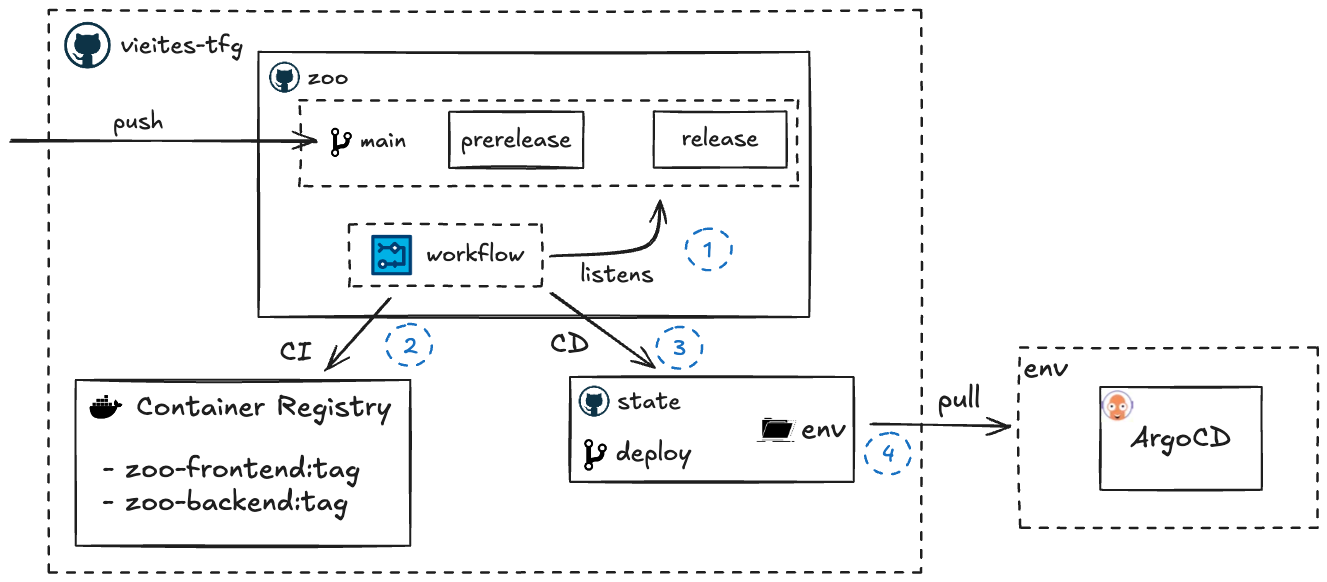
\includegraphics[width=13cm]{figuras/promotion}}
  \caption{Diagrama del proceso de promoción de entornos. Imagen creada con \href{https://excalidraw.com}{excalidraw.com}. También referenciado en la Sección \ref{sec:promotion}.}
  \label{fig:promotion}
\end{figure}


\section{helm-repository}
\label{subsec:helm}

Es una práctica habitual tener un repositorio con todas las Charts de Helm que utiliza el equipo de desarrollo. Esto permite tener un lugar centralizado para que los desarrolladores compartan y los usuarios encuentren aplicaciones para desplegar en Kubernetes.

Este repositorio tiene como finalidad lo que se acaba de comentar, funcionar como el lugar en el que se almacena la Chart de Helm de la aplicación de prueba.

La Figura \ref{fig:helm-repository} muestra que se ha creado una Chart \textit{umbrella} llamada \texttt{zoo}. Una Chart de este tipo funciona como una agrupación de más \textit{subcharts} que están interrelacionadas. Normalmente se utiliza este método para gestionar despliegues de aplicaciones complejas en Kubernetes.
La definición de la Chart \texttt{zoo} se puede ver en el Listing \ref{lst:umbrella}. En esta se indican las dependencias (\textit{subcharts}) que agrupa la Chart. Entre estas se encuentran las Charts propias de la aplicación, \texttt{zoo-frontend} y \texttt{zoo-backend}. Además, se puede ver que se utiliza una Chart ya definida en un repositorio conocido, perteneceinte a Bitnami\cite{bitnami}. De este repositorio se obtiene la Chart de MongoDB. De esta manera, se utiliza una Chart ya implementada y desarrollada por expertos, proporcionando muchas opciones de configuración y ofreciendo mucha más seguridad de lo que se tendría en el caso de crear una Chart de MongoDB propia para la aplicación.

\begin{listing}[!ht]
  \begin{minted}{yaml}
apiVersion: v2
name: zoo
description: Umbrella chart to deploy frontend, backend and mongo
version: 0.0.7
appVersion: "0.0.0"
dependencies:
  - name: zoo-frontend
    version: 0.0.0
    repository: file://charts/zoo-frontend
  - name: zoo-backend
    version: 0.0.0
    repository: file://charts/zoo-backend
  - name: mongodb
    repository: https://charts.bitnami.com/bitnami
    version: 15.0.0
    condition: mongo.internal.enabled
  \end{minted}
  \caption{Definición de la Chart umbrella de la aplicación}
  \label{lst:umbrella}
\end{listing}

También se puede observar en la Figura \ref{fig:helm-repository} los recursos que se crean para cada una de las \textit{subcharts} de la aplicación. Para más detalle en cuanto al funcionamiento de cada uno de los recursos, ver la Sección \ref{tech:k8s}.

Se detalla el proceso de desarrollo de la Chart de la aplicación en la Sección \ref{sec:chart}.

\begin{figure}
  \centerline{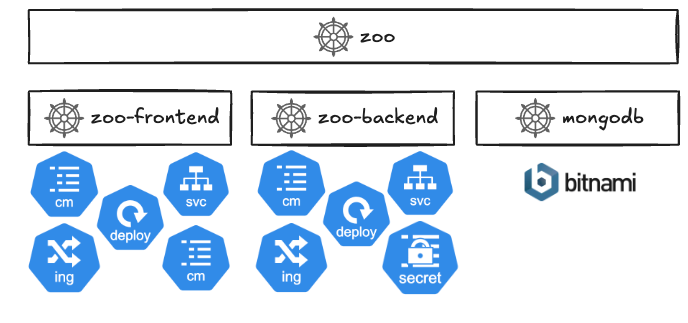
\includegraphics[width=13cm]{figuras/helm-repository}}
  \caption{Diagrama de organización de las Charts de la aplicación. Imagen creada con \href{https://excalidraw.com}{excalidraw.com}.}
  \label{fig:helm-repository}
\end{figure}

\section{state}
\label{subsec:state}

El repositorio de estado funciona como única fuente de verdad. Aquí se definen  los valores que pueblan la Chart de la aplicación. Se utiliza una herramienta llamada \texttt{helmfile}\cite{helmfile}. Esta permite integrar Charts de Helm y valores, aunque estos se encuentren en lugares diferentes. En la Figura \ref{fig:state} se muestra la estructura del repositorio de estado, incluyendo la rama principal y la rama de despliegue.

Se puede ver el archivo de configuración de \texttt{helmfile} en el Listing \ref{lst:helmfile}. Los archivos del apartado de \texttt{environments} indican el \textit{namespace} y la versión de la Chart que se va a utilizar. Los valores de las líneas 19-22 son aquellos que no dependen del entorno en el que se quiere desplegar, mientras que los de las líneas 23-26 sí que dependen del entorno, y se almacenan en un directorio dedicado a cada uno de ellos. En estos últimos archivos de valores dependientes del entorno se indica, por ejemplo, la \textit{tag} a utilizar de las imágenes de Docker.

\begin{longlisting}
  \begin{minted}{yaml}
  repositories:
  - name: helm-repository
    url: https://raw.githubusercontent.com/vieites-tfg/helm-repository/gh-pages/

environments:
  dev:
    values:
      - ./dev.yaml
  # ... otros entornos

---

releases:
  - name: zoo-{{ .Environment.Name }}
    namespace: {{ .Environment.Name }}
    chart: helm-repository/zoo
    version: {{ .Values.version }}
    values:
      - zoo-frontend.yaml
      - zoo-backend.yaml
      - mongodb.yaml
      - global.yaml
      - {{ .Environment.Name }}/zoo-frontend.yaml
      - {{ .Environment.Name }}/zoo-backend.yaml
      - {{ .Environment.Name }}/mongodb.yaml
      - {{ .Environment.Name }}/global.yaml
      - global:
          ghcrSecret:
            enabled: true
            password: {{ requiredEnv "CR_PAT" | quote }}
      - zoo-backend:
          mongo:
            root:
              user: {{ requiredEnv "MONGO_ROOT" | quote }}
              password: {{ requiredEnv "MONGO_ROOT_PASS" | quote }}
      - mongodb:
          auth:
            rootUser: {{ requiredEnv "MONGO_ROOT" | quote }}
            rootPassword: {{ requiredEnv "MONGO_ROOT_PASS" | quote }}
  \end{minted}
  \caption{Archivo de configuración de helmfile}
  \label{lst:helmfile}
\end{longlisting}

Un ejemplo de archivo de valores se puede observar en el Listing \ref{lst:values}. Como se ha comentado, el valor de la \textit{tag} se ve indicado en la línea 3, con el formato que se menciona en la Sección \ref{sec:promotion}.

\begin{listing}[!ht]
  \begin{minted}{yaml}
zoo-backend:
  image:
    tag: "69ab8a1e"
  mongo:
    service:
      name: "zoo-dev-mongodb"
  ingress:
    hostTemplate: "api-zoo-dev.example.com"
  \end{minted}
  \caption{Archivo de valores de zoo-backend en dev}
  \label{lst:values}
\end{listing}

En la Sección \ref{sec:cd} se explica cómo se especifica el entorno y, por lo tanto, los valores que se van a utilizar para poblar la Chart de la aplicación.

Este repositorio también es el lugar en el que se almacenan los archivos que definen los recursos que se van a desplegar en cada entorno. En la Figura \ref{fig:secrets} se puede ver la estructura que tiene uno de los directorios (\texttt{dev}) de la rama de despliegue del repositorio \textit{state}. La estructura de dicho directorio en la rama \texttt{deploy} es la misma para los directorios correspondientes a los demás entornos.

\begin{figure}[h]
  \centerline{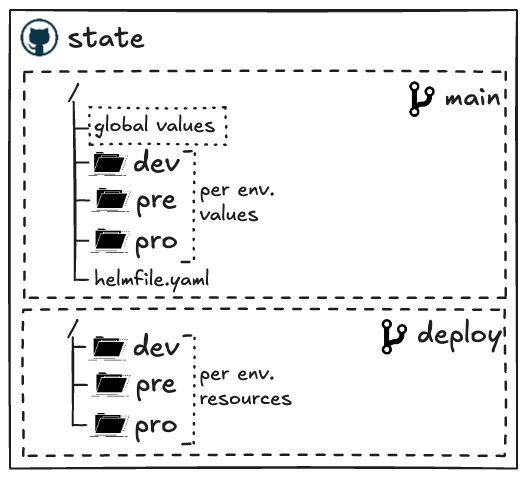
\includegraphics[width=12cm]{figuras/state}}
  \caption{Diagrama de la estructura del repositorio de estado. Imagen creada con \href{https://excalidraw.com}{excalidraw.com}.}
  \label{fig:state}
\end{figure}


\cleardoublepage
\chapter{Implementación del \textit{pipeline} con Dagger}
\label{chap:dagger}

Este capítulo describe la implementación del \textit{pipeline} con Dagger. Se parte de una versión inicial sin la herramienta, y se llega a un ciclo completo, plenamente integrado con esta herramienta. El objetivo es demostrar que Dagger aporta mayor flexibilidad a los desarrolladores para construir \textit{pipelines} de CI y CD, sin depender de tener un entorno de desarrollo ni de una configuración específica para ejecutarlos.

\section{CI}
\label{sec:ci}

Tras realizar una primera aproximación de la aplicación de prueba, el siguiente paso consiste en realizar el ciclo de CI. En este ciclo se realizan los tests de la aplicación, el \textit{linting}, es decir, verificar que el código cumpla ciertos estándares de estilo; y la publicación de imágenes de Docker y de paquetes NPM. Al principio se comenzó a implementar el ciclo completo sin el uso de Dagger. Se utilizó un \texttt{justfile} con los comandos necesarios para realizar tanto los tests como el \textit{linting} de los paquetes de la aplicación, y se crearon dos \textit{scripts}: uno para la publicación de imágenes y otro para la publicación de paquetes NPM. Además, se crea un Dockerfile para poder realizar las pruebas \textit{end-to-end} del \textit{frontend} con Cypress\cite{cypress}.

La desventaja con respecto al Dagger es evidente: \textit{scripts} y comandos que ``funcionan en mi máquina''. Siguiendo esta práctica, sería necesario que todo el equipo de desarrollo utilizara el mismo entorno de desarrollo, y aún así, no se garantizaría el funcionamiento del ciclo de CI, debido a posibles configuraciones que cada desarrollador haya hecho a su sistema que pueda diferir de las configuraciones de los demás. Con este método, los desarrolladores no tienen margen de maniobra en cuanto al sistema que deben utilizar.

Ahora se explica el diseño e implementación con Dagger del mismo ciclo de CI.

Una vez el ciclo de CI sin Dagger se ha realizado al completo, se pasó a traducir los scripts y comandos a un módulo de CI con Dagger, utilizando el SDK de Go.

En la Figura \ref{fig:dagger-ci} se puede comprobar la estructura de este módulo. Se ha optado por implementar un objeto principal \texttt{Ci}, el cual tiene la capacidad de hacer uso de cualquiera de los otros dos objetos customizados, uno específicamente diseñado para gestionar el \textit{frontend} y otro para el \textit{backend}. Este diseño concuerda con la propia estructura y filosofía del \textit{monorepo}: elementos separados que realizan tareas diferentes, pero que se interrelacionan desde un punto central (Lerna para el \textit{monorepo}, y el objeto \texttt{Ci} para el módulo).

\begin{figure}[h]
  \centerline{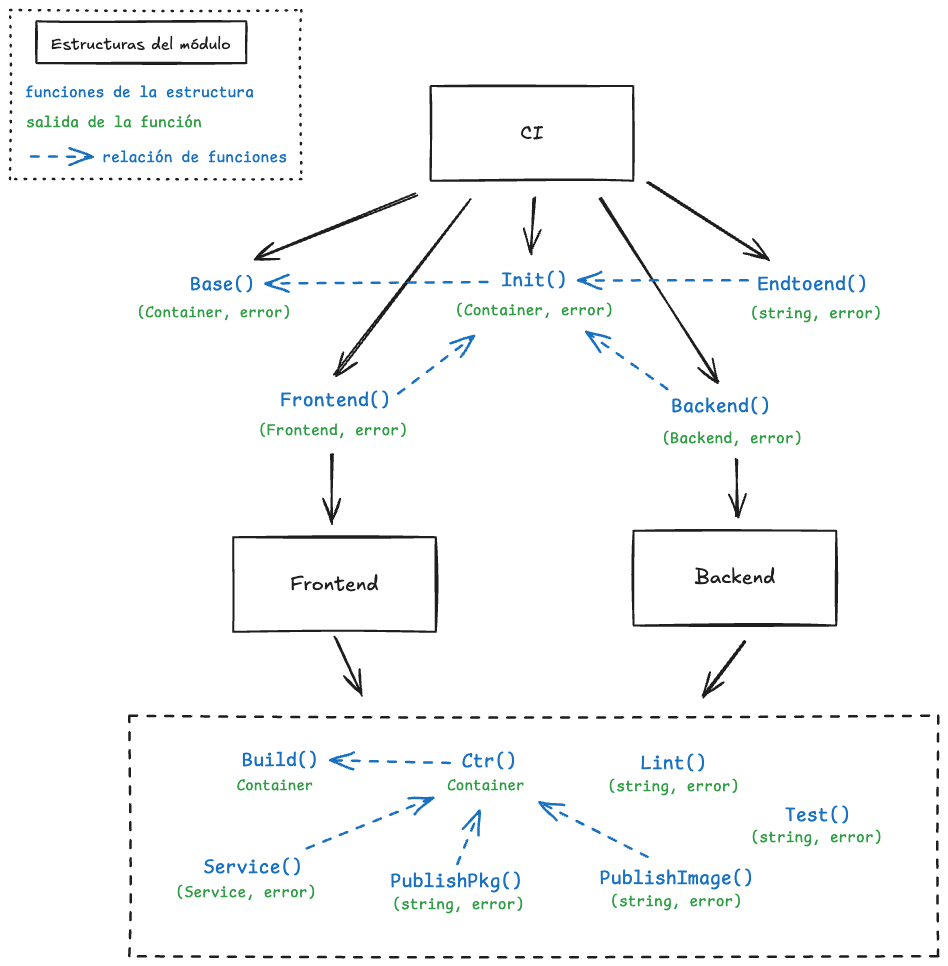
\includegraphics[width=12cm]{figuras/dagger-CI}}
  \caption{Diagrama del diseño del módulo de CI con Dagger. Imagen creada con \href{https://excalidraw.com}{excalidraw.com}}
  \label{fig:dagger-ci}
\end{figure}

Por lo tanto, la idea del diseño del módulo es la misma que la del \textit{monorepo}, tener un elemento principal desde el que hacer uso de cualquiera de los otros tipos customizados\cite{dagger-custom-types}, que se corresponden con los paquetes de la aplicación.

En Dagger se hace uso del ``encadenamiento''. Esto permite llamar a las funciones de los objetos que devuelven las propias funciones. Así, se puede llamar a la función del objeto principal del módulo que devuelve el objeto \texttt{Backend}, y se tendrá acceso a las funciones que están definidas para este paquete.

Para entender cómo funciona, se explicará un ejemplo sencillo con pseudocódigo del propio módulo. En el Listing \ref{lst:chaining-code} se puede ver un ejemplo de dos funciones del módulo de CI (se han escrito comentarios de lo que se hace en el código para reducir su tamaño). La primera función corresponde con el objeto principal del módulo. Este construye la imagen base y posteriormente crea un objeto \texttt{Backend}, el cual devuelve como referencia al final de la función. El hecho de que este objeto sea devuelto por la función, permite acceder a las funciones que este tiene definidas.

Una función definida para \texttt{Backend} es \texttt{Test}, que aparece justo después. En esta se utiliza la imagen base que se ha pasado como parámetro en la construcción del objeto. Se ejecuta dentro del contenedor que define dicha imagen el comando que permite correr los tests del paquete \textit{backend} de la aplicación. Como se puede comprobar, se utiliza Lerna para ejecutar el \textit{script} \texttt{test}, definido en el \texttt{package.json} del paquete correspondiente, indicado mediante el parámetro \textit{scope}.

\begin{longlisting}
  \begin{minted}{go}
// Ci (main.go)

type Ci struct {
	// +required
	SecEnv  *dagger.Secret
	secrets secrets
}

func (m *Ci) Backend(
ctx context.Context,
// +defaultPath="/"
src *dagger.Directory,
) (*Backend, error) {
  base, _ := m.Init(ctx, src)

  // Se obtienen las claves y los valores de los secretos para
  // el *backend*.

  return &Backend{
    Name:    "backend",

    // Imagen base, con todo lo necesario para ejecutar los
    // comandos que se precise.
    Base:    base,

    // Claves y valores de los secretos obtenidos antes.
    Secrets: SecMap{Keys: keys, Values: values},
  }, nil
}

// Backend (backend.go)

func (m *Backend) Test(ctx context.Context) (string, error) {
  return m.Base.
    WithExec([]string{"lerna", "run", "test", "--scope", "@vieites-tfg/zoo-backend"}).
    Stdout(ctx)
}

\end{minted}
\caption{Funciones del módulo de Dagger de CI.}
\label{lst:chaining-code}
\end{longlisting}

La manera en la que se ejecuta a través de un comando la cadena de funciones anterior es como aparece en el Listing \ref{lst:chaining-command}. El comando se realiza en el directorio de trabajo del módulo de CI. Se hace una llamada a Dagger, se pasan los valores requeridos por el módulo, los cuales se indican en la definición del objeto principal; y finalmente se empieza a llamar a las funciones que tiene cada uno de los objetos. A las funciones se las llama en formato ``kebab-case'', aunque en el propio código estén en ``camelCase''. Por lo tanto, primero se realiza la llamada a la función \texttt{backend} y, posteriormente, sabiendo que esta función devuelve un tipo \texttt{Backend}, se llama a la función \texttt{test} que este tiene definida.

\begin{listing}[!ht]
  \begin{minted}{bash}
dagger call --sec-env=file://../../.env backend test
\end{minted}
\caption{Encadenamiento de funciones del módulo de CI.}
\label{lst:chaining-command}
\end{listing}

De esta manera se puede lanzar la función que se prefiera de cualquiera de los paquetes. También, esta estructura y diseño del módulo facilita la escalabilidad de la aplicación, permitiendo añadir fácilmente más paquetes en el caso de ser necesario. Lo único que habría que hacer sería crear un objeto nuevo con funciones para las tareas que se quieran realizar en este, y añadir una función en el objeto principal del módulo que devuelva el nuevo objeto creado para el paquete.

Junto con la ejecución de los tests y del \textit{linter}, se añade también al módulo la posibilidad de levantar por separado cada uno de los paquetes. Esto quiere decir que se permite acceder de manera local a los servicios de los paquetes, la página web por un lado y la API por el otro.

Antes de implementar esa lógica en el módulo de CI, se desarrolla lo necesario para conseguir levantar la aplicación entera de la manera más sencilla posible. En este caso, se utiliza un \texttt{Dockerfile} con varios pasos, en los cuales se construye y se prepara la imagen para la ejecución de cada uno de los paquetes. Esto se consigue con construcciones \textit{multi-stage}, un ejemplo de esto se encuentra en el Listing \ref{lst:dockerfile}.

Con el \texttt{Dockerfile} anterior y con la construcción de un \texttt{docker-compose.yaml}, se consigue levantar la aplicación de manera local. Tras conseguir esto, se traduce de nuevo la lógica al módulo de Dagger. Se crea en cada uno de los objetos del módulo una función \texttt{service}, que permiten levantar los paquetes por separado y acceder a ellos de manera local. Gracias a estas funciones es posible realizar los tests \textit{end-to-end} de la aplicación, donde una única función es capaz de realizar los siguientes pasos:

\begin{itemize}
  \item Tests y \textit{linting} de cada uno de los paquetes.
  \item Levantar los servicios de los paquetes, permitiendo su comunicación de manera interna.
  \item Correr los tests de la aplicación con Cypress.
\end{itemize}

Todo lo anterior integrado en el módulo y ejecutado con una única llamada a una función del objeto principal de la aplicación.

Aquí es donde realmente se ve la potencia de Dagger. Todo se programa en un lenguaje conocido para el desarrollador, con sintaxis que no depende del sistema en el que se está desarrollando y sin la aparición de problemas relacionados con el entorno de ejecución, ya que funciona independientemente del sistema. Esto es gracias a ejecutar todo sobre un \textit{runtime} de OCI, como Docker. Para realizar todo lo anterior sin Dagger, habría que: lanzar los comandos de Lerna de manera local, levantar los servicios con Docker Compose y correr los tests de Cypress con un \texttt{Dockerfile} específico para la causa. Y aún haciendo todo esto, no se tendría la flexibilidad de realizar pruebas y obtener \textit{logs} que se tiene con Dagger. Además, Dagger permite acceder al contenedor en cualquier momento de la ejecución del \textit{pipeline}.

\section{CD}
\label{sec:cd}

El ciclo de CD involucra: la construcción de los recursos de Kubernetes, el encriptado de los secretos y la publicación de todos los manifiestos necesarios en el repositorio de estado.

Para comenzar con este ciclo, se crearon un par de \textit{scripts}, uno que permitía construir las imágenes de Docker y su publicación y otro que facilitaba la publicación de los paquetes NPM. Esto tiene las desventajas ya comentadas, son \textit{scripts} que se ejecutan de manera local y que, por lo tanto, dependen del entorno en el que se ejecutan. En el caso de cambiar de entorno de desarrollo, sería necesario crear nuevos \textit{scripts} o acomodarlos al nuevo entorno. Esto solo trae problemas innecesarios a los desarrolladores, que se tienen que centrar en solucinar estos inconvenientes, externos a la finalidad del desarrollo de la aplicación en sí.

Tras crear los \textit{scripts} anteriores, se pasó a la construcción de las Charts de Helm de la aplicación. Se diseñó la estructura de las Charts y los componentes que iban a tener cada uno de los servicios de la aplicación. Entonces se definieron todos los recursos con Helm y se realizaron pruebas hasta que finalmente todo funcionaba como se esperaba.

La construcción de las Charts era necesario realizarlo tras ser capaz de publicar las imágenes de Docker al Container Registry. Esto es porque Kubernetes utiliza imágenes construidas que obtiene de cualquier registro que se le indique, no se le puede pasar un \textit{Dockerfile} para que construya la imagen.

Todo el proceso de creación de las Charts se ha realizado en local, utilizando comandos de Helm. Una vez comprobada la funcionalidad de esta, se procedió a la separación de responsabilidades: un repositorio para las Charts por un lado (\texttt{helm-repository}), y otro repositorio con los valores que pueblan las Charts por otro lado (\texttt{state}). Esto facilita el desarrollo y mantenimiento de las Charts. Además, se tiene una única fuente de verdad para obtener los valores.

Con los distintos repositorios creados, es necesario utilizar la herramienta \texttt{helmfile} para integrar Charts y valores. El archivo de configuración de esta herramienta se incluye en el repositorio de estado, manteniendo así la norma de tener toda la gestión de valores en un mismo lugar.

Así, ya es posible desplegar la aplicación utilizando Kubernetes. Lo siguiente es hacer uso de Dagger para permitir realizar el despliegue. Se comienza utilizando un método \textit{push} de despliegue. En el propio módulo de Dagger que se creó inicialmente, se utiliza \texttt{helmfile} para desplegar la aplicación en un \textit{cluster} de KinD. No existe ArgoCD, ni varios entornos. Por ahora es sencillo y directo, se crea un \textit{cluster} con un módulo de KinD para Dagger, y se ejecuta el comando de \texttt{helmfile} necesario para desplegar la aplicación.

A continuación se decide emplear el método \textit{pull}, ya comentado, donde existe una herramienta que es la que se encarga de obtener los recursos que se van a desplegar. Esa herramienta es ArgoCD. El módulo de CD de Dagger pasa de desplegar la aplicación a ser el encargado de publicar en la rama \texttt{deploy} del repositorio \texttt{state} los recursos que se van a desplegar en cada entorno. Esto implica

\begin{enumerate}
  \item Realizar el \textit{template} de los recursos con \texttt{helmfile}, es decir, mostrar el renderizado de estos pero sin desplegarlos.
  \item Obtener los secretos y encriptarlos.
  \item Crear los archivos que dice a ArgoCD cómo desencriptar los secretos,
  \item Publicar todo en la rama de despliegue del repositorio de estado.
\end{enumerate}

Tras tener en funcionamiento el módulo, se procede a crear el \textit{workflow} de GitHub, cuyo funcionamiento se explica en la Sección \ref{sec:promotion}. En resumen, se encarga de ejecutar los módulos de CI y CD, ejecutando los tests \textit{end-to-end} previamente a la publicación de las nuevas imágenes de Docker y actualizando el repositorio de estado con la definición de los recursos en el entorno que proceda, utilizando las nuevas imágenes creadas.

De esta manera, se integra todo lo que se ha creado:

\begin{itemize}
  \item Los módulos de Dagger de CI y de CD.
  \item Las Charts de Helm y valores.
  \item Los \textit{clusters} de KinD con los entornos levantados, con ArgoCD instalado en cada uno de ellos.
  \item Un \textit{workflow} de GitHub que enlaza todo lo anterior.
\end{itemize}

\cleardoublepage
\chapter{Exemplos (eliminar capítulo na versión final)}

\section{Un exemplo de sección}
Esta é {\it letra cursiva}, esta é {\bf letra negrilla}, esta é \underline{letra subrallada}, e esta é {\tt letra curier}. Letra {\tiny tiny}, {\scriptsize scriptsize}, {\small small}, {\large large}, {\Large Large}, {\LARGE LARGE} e moitas más. Exemplo de fórmula: $a=\int_o^\infty f(t)dt$.  E agora unha ecuación aparte:

\begin{equation}
S=\sum_{i=0}^{N-1} a_i^2 .
\label{mi_ecuacion}
\end{equation}

As ecuaciones se poden referenciar: ecuación (\ref{mi_ecuacion}).

\subsection{Un exemplo de subsección}
O texto vai aquí.
\subsection{Otro exemplo de subsección}
O texto vai aquí.
\subsubsection{Un exemplo de subsubsección}
O texto vai aquí.
\subsubsection{Un exemplo de subsubsección}
O texto vai aquí.
\subsubsection{Un exemplo de subsubsección}
O texto vai aquí.
\section{Exemplos de figuras e cadros}

A figura número \ref{enlace1}.

O cadro (taboa) número \ref{enlace2}.

\begin{figure}
\centerline{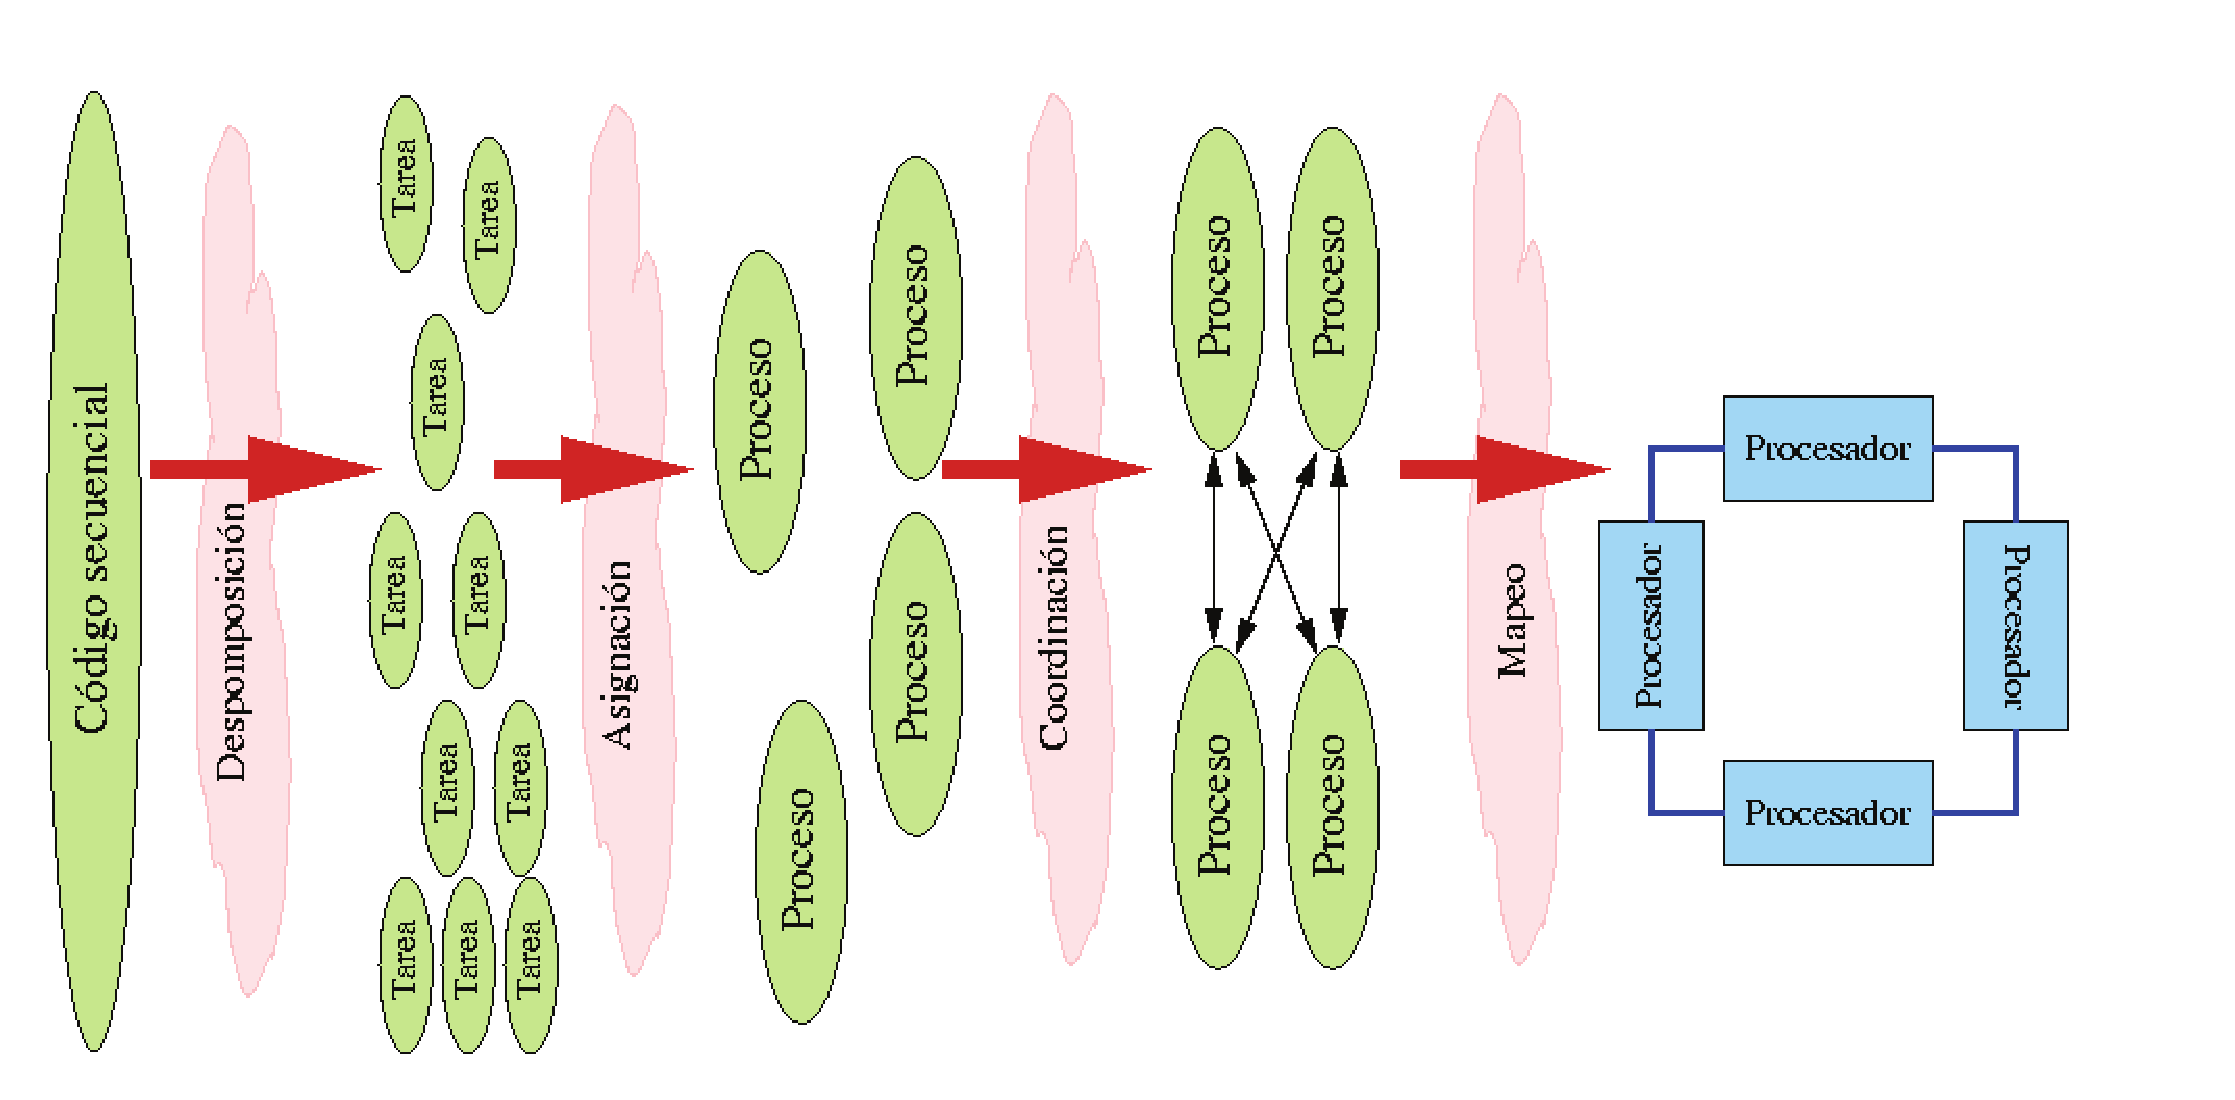
\includegraphics[width=15cm]{figuras/figura01.eps}}
\caption{Esta é a figura de tal e cal.}
\label{enlace1}
\end{figure}

\begin{table}
\begin{center}
\begin{tabular}{|l||r|c|} \hline
Izquierda & Derecha & Centrado  \\ \hline\hline
ll & r & cccc \\ \hline
llll & rrr & c \\ \hline
\end{tabular}
\caption{Esta é a táboa de tal e cal.}
\label{enlace2}
\end{center}
\end{table}

\section{Exemplos de referencias á bibliografía}
% Este é un exemplo de referencia a un documento descargado da web \cite{cuda}. E este é un exemplo de referencia a unha páxina da wikipedia \cite{cdma}. Agora un libro \cite{gonzalez} e agora unha referencia a un artigo dunha revista \cite{patricia}. Tamén se poden pór varias referencias á vez \cite{cuda,gonzalez}.

\section{Exemplos de enumeracións}

Con puntos:

\begin{itemize}
\item Un.
\item Dous.
\item Tres.
\end{itemize}

Con números:

\begin{enumerate}
\item Catro.
\item Cinco.
\item Seis.
\end{enumerate}

Exemplo de texto verbatim:

\begin{verbatim}
O texto        verbatim 
     se visualiza tal
            como se escribe
\end{verbatim}

Exemplo de código C:

\lstset{language=C}

\begin{lstlisting}
#include <math.h>
main()
{  int i, j, a[10];
   for(i=0;i<=10;i++) a[i]=i; // comentario 1
   if(a[1]==0) j=1; /* comentario 2 */
   else j=2;
}
\end{lstlisting}

Exemplo de código Java:

\lstset{language=java}

\begin{lstlisting}
class HelloWorldApp {
    public static void main(String[] args) {
        System.out.println("Hello World!"); // Display the string.
    }
}
\end{lstlisting}



%
% Engadir os capitulos que fagan falta
%
\cleardoublepage
\chapter{Conclusiones y posibles ampliaciones}

%O traballo describe o grao de cumprimento dos obxectivos. Posibles vías de mellora.

A lo largo del trabajo se explica todo el proceso de diseño e implementación de: la aplicación de prueba, las Charts de Helm que permiten el despliegue de la aplicación en Kubernetes y los módulos de Dagger para los ciclos de CI y CD. Esto último es la razón por la que se ha hecho este trabajo.

Crear un módulo de Dagger implica tener conocimientos de programación, pero también de creación de entornos aislados, como son los contenedores de Docker. Además, requiere estudiar la API que proporciona, la cual es más intuitiva en el caso de tener los conocimientos que se acaban de mencionar. Por lo tanto, es una herramienta que tiene una curva de aprendizaje moderada, sobre todo inicialmente.

Una vez se comienza el desarrollo de los módulos, el hecho de que se utilice un lenguaje de programación como Go facilita mucho la gestión de la lógica de programación, permitiendo crear funciones que se pueden llamar desde cualquier otro lugar dentro del módulo. Tras tener más conocimiento de la herramienta, la dificultad de desarrollar módulos de CI y CD radica más en el diseño de los propios módulos que en la programación en sí.

La capacidad de Dagger para crear módulos de CI/CD de manera programática facilita en gran medida el mantenimiento de estos a largo plazo, ya que no se utilizan diferentes herramientas o tecnologías que puedan depender del entorno de desarrollo. A lo largo de la implementación de los módulos, el programador se da cuenta de las ventajas que tiene poder centralizar toda la lógica de programación. Cabe mencionar la gran portabilidad que proporciona Dagger gracias a que se ejecuta sobre un \textit{runtime} de OCI, lo cual permite ejecutar los módulos creados con esta herramienta de manera local en una gran variedad de entornos de desarrollo. Además, se encuentran de manera pública módulos en el Daggerverse, los cuales están implementados por otros desarrolladores. Estos se pueden integrar muy fácilmente en otros módulos en desarrollo.

Por otro lado, la gestión que realiza Dagger de la caché permite al desarrollador reducir en gran medida los tiempos de ejecución de funciones que se lanzan de manera repetitiva a lo largo del proceso de desarrollo de la aplicación. Un ejemplo de esto se ha visto en las pruebas realizadas \ref{chap:pruebas}.

Todo lo mencionado anteriormente hace de Dagger una excelente opción para crear módulos de este tipo para cualquier aplicación. Aprender a utilizar esta herramienta puede facilitar en gran medida la implementación, el mantenimiento, la portabilidad, la flexibilidad, la escalabilidad y la reproducibilidad de \textit{pipelines} de CI/CD para una aplicación.

\section{Vías de mejora}

A continuación, se mencionan elementos que se pueden mejorar en un futuro con respecto al trabajo realizado:

\begin{itemize}
  \item Posible mejora del diseño de los módulos de CI/CD.
  \item Añadir más funcionalidades a la aplicación de prueba.
  \item Despliegue de la aplicación en proveedores en la nube, en vez de levantar todos los \textit{clusters} de KinD de manera local.
  \item Gestión de secretos más avanzada.
  \item Añadir una herramienta de monitorización y observabilidad de métricas de la aplicación, tales como DataDog\cite{datadog} o Prometheus\cite{prometheus}.
  \item Escalado horizontal\cite{horizontal}, con el fin de distribuir la carga entre múltiples instancias, mejorando la escalabilidad, la tolerancia a fallos y la disponibilidad de la aplicación.
  \item Análisis de imágenes de Docker y \texttt{Dockerfiles}, para mayor seguridad, empleando herramientas como Trivy\cite{trivy}.
  \item Realización de encuestas o entrevistas a más desarrolladores que prueben la herramienta, con el fin de obtener más \textit{feedback} y validar con mayor firmeza las conclusiones a las que se han llegado en este trabajo.
\end{itemize}


% Aquí empezan os apéndices
\appendix
\cleardoublepage
\chapter{Manuais técnicos}

En función do tipo de Traballo e metodoloxía empregada, o contido poderase dividir en varios documentos. En todo caso, neles incluirase toda a información precisa para aquelas persoas que se vaian encargar do desenvolvemento e/ou modificación do Sistema (por exemplo código fonte, recursos necesarios, operacións necesarias para modificacións e probas, posibles problemas, etc.). O código fonte poderase entregar en soporte informático en formatos PDF ou postscript.
\cleardoublepage
\chapter{Manuais de usuario}

Incluirán toda a información precisa para aquelas persoas que utilicen o Sistema: instalación, utilización, configuración, mensaxes de erro, etc. A documentación do usuario debe ser autocontida, é dicir, para o seu entendemento o usuario final non debe precisar da lectura doutro manual técnico.

\cleardoublepage
\chapter{Licenza}
Se se quere pór unha licenza (GNU GPL, Creative Commons, etc), o texto da licenza vai aquí.


\cleardoublepage
\markboth{BIBLIOGRAFÍA}{BIBLIOGRAFÍA}
\addcontentsline{toc}{chapter}{Bibliografía}


\begin{thebibliography}{99}
% EXEMPLO DE DOCUMENTO DESCARGADO DA WEB
\bibitem{cuda} Nvidia CUDA programming guide. Versión 2.0, 2010. Dispoñible en {\it http://www.nvidia.com}.

% EXEMPLO DE PÁXINA DA WIKIPEDIA
\bibitem{cdma} Acceso múltiple por división de código. Artigo da wikipedia ({\it http://es.wikipedia.org}). Consultado o 2 de xaneiro do 2010.

% EXEMEPLO DE LIBRO
\bibitem{gonzalez} R.C. Gonzalez e R.E. Woods, {\it Digital image processing}, 3ª edición, Prentice Hall, New York, 2007.

% EXEMPLO DE ARTIGO DE REVISTA
\bibitem{patricia} P. González, J.C. Cartex e T.F. Pelas, ``Parallel computation of wavelet transforms using the lifting scheme'', {\it Journal of Supercomputing}, vol. 18, no. 4, pp. 141-152, junio 2001.
\end{thebibliography}



\end{document}
